\documentclass[%
candidate,     % тип документа
href,        % использовать пакет hyperref для создания гиперссылок
colorlinks,  % цветные гиперссылки
%times,      % шрифт Times как основной
%facsimile,   % отображать факсимиле диссертанта и ученого секретаря
]{disser}

\usepackage[%
  a4paper, mag=1000,
  left=2.5cm, right=1cm, top=2cm, bottom=2cm, headsep=0.7cm, footskip=1cm
]{geometry}

\usepackage[intlimits]{amsmath}
\usepackage{amssymb,amsfonts}
\usepackage[T2A]{fontenc}
\usepackage[utf8]{inputenc}
\usepackage[autostyle]{csquotes}
\usepackage[english,russian]{babel}
\usepackage{tabularx}
\usepackage{multirow}
\usepackage{relsize}
\ifpdf\usepackage{epstopdf}\fi

\usepackage[%
    backend=biber,
    bibencoding=utf8,
    sorting=none,
    style=numeric,
    citestyle=numeric-comp,
    language=auto,
    autolang=other,
    sortcites=true,
    doi=true,
    isbn=false,
    maxbibnames=6,
    defernumbers=true
]{biblatex}
\addbibresource{references.bib}
\defbibheading{authorcited}{\nsection{Публикации автора по теме диссертации}}
\defbibheading{cited}{\nsection{Цитированная литература}}

\AtNextCitekey{\!}

% Номера страниц снизу и по центру
\pagestyle{footcenter}
\chapterpagestyle{footcenter}

% Путь к файлам с иллюстрациями
\graphicspath{{fig/}}

\showboxdepth=5
\showboxbreadth=5

\begin{document}
% Включение файла с общим текстом диссертации и автореферата
% (текст титульного листа и характеристика работы).
% Общие поля титульного листа диссертации и автореферата
\institution{Федеральное государственное бюджетное учреждение науки \\ Институт системного программирования им. В.П.~Иванникова \\ Российской академии наук (ИСП РАН)}

\topic{Методы декомпозиции систем и моделирования окружения программных модулей для верификации Си-программ}
\author{Захаров Илья Сергеевич}

\specnum{05.13.11}
\spec{математическое и программное обеспечение\\ 
вычислительных машин, комплексов и компьютерных сетей}

\sa{Петренко Александр Константинович}
\sastatus{д.~ф.-м.~н., проф.}

\city{Москва}
\date{\number\year}

\mkcommonsect{objective}{Цели и задачи работы.}{%

{\bf Цель работы} --- развитие методов верификации крупных программных систем на языке программирования Си с использованием инструментов верификации моделей программ при помощи автоматизации декомпозиции системы на модули и синтеза моделей их окружения для сокращения трудоемкости и сроков верификации.

Для достижения поставленной цели были решены следующие задачи:
\begin{enumerate}
    \item Исследовать существующие подходы к применению инструментов верификации моделей программ для проверки требований к Си-программам и выявить проблемы, препятствующие расширению применения этих подходов на практике.
    \item Разработать архитектуру системы верификации Си-программ, выполняющей генерацию и решение набора верификационных задач при помощи автоматизированной декомпозиции системы на модули и синтеза моделей окружения модулей.
    \item Разработать метод автоматизированной декомпозиции Си-программ на модули.
    \item Разработать метод автоматизированного синтеза моделей окружения модулей, позволяющий адаптировать процесс синтеза для проверки разных видов требований и программ.
    \item Реализовать систему верификации моделей Си-программ на основе разработанных архитектуры и методов, оценить реализацию системы верификации на практике.
\end{enumerate}
}

\mkcommonsect{novelty}{Научная новизна.}{%

Научной новизной обладают следующие результаты работы:
\begin{itemize}
\item Метод автоматизированной декомпозиции Си-программ на модули.
\item Метод спецификации моделей окружения модулей Си-программ на основе композиции систем переходов и доказательство теоремы об изоморфизме множеств достижимых ошибочных состояний спецификации и результата ее трансляции на язык Си.
\item Метод автоматизированного синтеза моделей окружения модулей, позволяющий адаптировать процесс синтеза для проверки разных видов требований и программ.
\end{itemize}
}

\mkcommonsect{method}{Методология и методы исследования.}{%

Результаты диссертации были получены с использованием методов и моделей, применяемых при проведении верификации моделей программ. Математическую основу данной работы составляют теория графов, теория множеств, математическая логика и системы переходов.
}


\mkcommonsect{results}{Положения, выносимые на защиту.}{%

\begin{itemize}
    \item Метод автоматизированной декомпозиции Си-программ на модули.
    \item Метод спецификации моделей окружения модулей на основе композиции систем переходов.
    \item Метод автоматизированного синтеза моделей окружения модулей, позволяющий адаптировать процесс синтеза для проверки разных видов требований и программ.
\end{itemize}

На основе предлагаемых методов была реализована система верификации Klever, предназначенная для проверки требований к программным системам на языке программирования Си с расширениями GNU методом верификации моделей программ. Продемонстрировано, что разработанная архитектура системы верификации позволяет проводить верификацию на различных многоядерных и распределенных вычислительных системах.

}

\mkcommonsect{aprob}{Степень достоверности и апробация результатов.}{%

Основные результаты работы обсуждались на конференциях:
\begin{itemize}
\item 55-я научная конференция МФТИ (г.~Москва, 2012 год).
\item Международная научная конференция студентов, аспирантов и молодых учёных «Ломоносов-2013» (г.~Москва, 2013 год).
\item 7-й весенний/летний коллоквиум молодых исследователей в области
программной инженерии (SYRCoSE, г.~Казань, 2013 год).
\item 10-я конференция разработчиков свободных программ (OSSDEVCONF, г.~Калуга, 2013 год).
\item Международная Ершовская конференция по информатике\linebreak (PSI:~Perspectives of System informatics, г.~ Санкт-Петербург, 2014 год).
\item 5-й международный семинар Linux Driver Verification (г.~Москва, 2015 год).
\item 10-я летняя школа Microsoft Research (г.~Кембридж, Великобритания,
2015 год).
\item 1-й международный семинар, посвященный инструменту CPAchecker \\(г.~Пассау, Германия, 2016 год).
\item 2-й международный семинар, посвященный инструменту CPAchecker \\(г.~Падерборн, Германия, 2017 год).
\item 5-я Международная научно-практическая конференция «Инструменты и методы анализа программ» (г.~Москва, 2017 год).
\item Международная Ершовская конференция по информатике\linebreak (PSI:~Perspectives of System informatics, г.~Москва, 2017 год).
\item 5-я научно-практическая конференция OS DAY (г.~Москва, 2018 год).
\item Научно-практическая открытая конференция ИСП РАН им. В.П.~Иванникова (г.~Москва, 2018 год).
\item Семинар ИСП РАН (г.~Москва, 2018 год).
\end{itemize}
}

\mkcommonsect{pub}{Публикации и зарегистрированные программы.}{%

% Публикации
По теме исследования опубликовано 11 работ \parencite{Syrcose,EnvTrudy,configurable:Trudy,Zakharov2015,ZakharovEnv2015,ZakharovEnvPsi,subsystems:Trudy,survey:new,klever:new,Novikov:2018:ISOLA,Zakharov:2018:ISPRAS} из них 9 в изданиях перечня ВАК~\cite{EnvTrudy,configurable:Trudy,Zakharov2015,ZakharovEnv2015,ZakharovEnvPsi,subsystems:Trudy,survey:new,klever:new,Novikov:2018:ISOLA} и 6 входят в международную систему цитирования Scopus~\cite{Zakharov2015,ZakharovEnv2015,ZakharovEnvPsi,survey:new,klever:new,Novikov:2018:ISOLA}.
В совместных работах~\cite{configurable:Trudy,Zakharov2015} личный вклад автора заключается в описании метода моделирования окружения, а в работах ~\cite{EnvTrudy,ZakharovEnv2015,ZakharovEnvPsi} в описании реализации метода моделирования окружения в системе верификации LDV~Tools.
В совместных работах~\cite{subsystems:Trudy,klever:new,Novikov:2018:ISOLA} личный вклад автора состоит в описании методов декомпозиции программ на модули, а также спецификации и синтеза моделей окружения.

% Патенты
В ходе выполнения работы было получено 4 свидетельства о государственной регистрации программ для ЭВМ:
\begin{enumerate}
\item Свидетельство о государственной регистрации программы для ЭВМ \\№~2015662948: «Программный компонент решения задач верификации посредством использования инфраструктуры облачного сервиса».
\item Свидетельство о государственной регистрации программы для ЭВМ \\{№~2017660773}: «Klever Linux Kernel Verification Objects Generator».
\item Свидетельство о государственной регистрации программы для ЭВМ \\№~2017660774: «Klever Environment Model Generator for Linux Kernel\linebreak Modules».
\item Свидетельство о государственной регистрации программы для ЭВМ \\№~2017660776: «Klever Verification Scheduler».
\end{enumerate}
}

\mkcommonsect{contrib}{Личный вклад автора.}{%

Все представленные в диссертации результаты получены лично автором.
\pagebreak
}

\mkcommonsect{struct}{Структура и объем диссертации.}{%

Диссертация состоит из введения, обзора литературы, 5 глав, заключения и библиографии.
Общий объем диссертации 157 страниц, включая 10 рисунков и 14 таблиц.
Библиография включает 143 наименования на 18 страницах.
}

\thispagestyle{empty}
\begin{center}
\large{
Федеральное государственное бюджетное учреждение науки \\ Институт системного программирования им. В.П. Иванникова \\ Российской академии наук (ИСП РАН)}
\end{center}
\vspace{8mm}
\begin{flushleft}
\textbf{Направление подготовки}: 09.06.01\\
\textbf{Направленность (профиль) подготовки}: 05.13.11\\
\textbf{Форма обучения}: очная\\
\end{flushleft}
\vspace{10mm}
\begin{center}
\textbf{
НАУЧНЫЙ ДОКЛАД\\
ОБ ОСНОВНЫХ РЕЗУЛЬТАТАХ ПОДГОТОВЛЕННОЙ\\
НАУЧНО-КВАЛИФИКАЦИОННОЙ РАБОТЫ (ДИССЕРТАЦИИ)}
Метод масштабируемой модульной статической верификации программ на языке Си с расширениями GNU
\end{center}
\vspace{10mm}
\begin{flushleft}
\hspace*{.5\linewidth}\textbf{Аспирант}: Захаров Илья Сергеевич\\
\hspace*{.5\linewidth}\hrulefill\\
\hspace*{.5\linewidth}\textbf{Научный руководитель}:\\
\hspace*{.5\linewidth}Петренко Александр Константинович,\\
\hspace*{.5\linewidth}д.~ф.-м.~н., проф.\\
\hspace*{.5\linewidth}\hrulefill\\
\end{flushleft}
\vspace{15mm}
\begin{center}
Москва 2018
\end{center}
\clearpage

\nsection{Общая характеристика работы}

% Актуальность работы
\actualitysection
\actualitytext

% Цели и задачи диссертационной работы
\objectivesection
\objectivetext

% Научная новизна
\noveltysection
\noveltytext

% Теоретическая и практическая значимость
\valuesection
\valuetext

% Положения, выносимые на защиту
%\resultssection
%\resultstext

% Степень достоверности и апробация результатов
%\approbationsection
%\approbationtext

% Публикации
\pubsection
\pubtext

% Личный вклад автора
%\contribsection
%\contribtext

% Структура и объем диссертации
\structsection
\structtext

\nsection{Содержание работы}

\nsubsection{Глава 1}
% Ожидается в сумме 10 страниц

% На что нацелен обзор 
Технология проверки моделей программного обеспечения и статической верификации в частности активно развивается и рассмотреть все возможные направления и методы, существующие в данной области науки, достаточно трудно и не является целью данной главы.
Тем более, что существует достаточно много работ, которые описывают историю возникновения методов и сами методы анализа моделей и программ, а также представляют сравнение данного направления с другими методами верификации программ~\cite{Vorobyov2010ComparingMC, DSilva:2008:SAT, Clarke:2008:BMC, HandbookMC}.
Цель же данного обзора --- рассмотреть особенности и проблемы практического применения методов и инструментов статической верификации к программам из индустрии, разработанных на языке Си с расширениями GNU.
Ниже будет очерчена область применимости инструментов статической верификации и названы основные ограничения существующих инструментов.
Также будут рассмотрены существующие успехи в преодолении проблемы масштабируемости инструментов статической верификации и проверки моделей.

\nsubsubsection{Инструменты статической верификации программ}
% Что понимается под статической верификацией
Методы статической верификации сочетают в себе такие направления, как абстрактная интерпретация~\cite{Cousot:1977:AIU}, символьное выполнение~\cite{Boyer:1975:SFS}, предикатная абстракция~\cite{Graf:1997:CAS}. 
Инструменты статической верификации автоматически извлекают модель программы из ее исходного кода. Верифицируемая модель программы по построению содержит те же ошибки, что и исходный код, но может быть менее точной. 
При верификации данной модели используются формальные методы проверки моделей~\cite{Biere03boundedmodel} или уточнение абстракции по контр-примеру~\cite{Clarke:2003:CAR}.

% SV-COMP rules
С 2012 года в рамках конференции TACAS происходит ежегодное соревнование инструментов статической верификации \mbox{SV-COMP 2017}.
Соревнования нацелены на сравнение точности и производительности существующих инструментов статической верификации на подготовленных заранее наборах программ.
Год от года число команд разработчиков растет.
В 2012 году их было около десятка, а в \mbox{SV-COMP 2017} году в рамках соревнований команд стало уже 32~\cite{Beyer:2017:SVV}.
Правила соревнований во многом определяют возможности инструментов и их интерфейс.

% Front-end
Инструменты статической верификации верифицируют модель, построенную на основе исходного кода целевой программы.
Для верификации программ на различных языках используется внутреннее представление, не зависящее от конкретного языка.
Например, инструмент статической верификации \mbox{Corral} использует инфраструктуру \mbox{SMACK} для трансляции программ во внутреннем представлении \mbox{LLVM} в программу на языке \mbox{Boogie}~\cite{tacas2015-hcelqr}.
А для работы с программами на языке Си в инструменте статической верификации \mbox{CPAchecker}~\cite{Beyer:2011:CTC} используется парсер Eclipse CDT, хотя инструмент также поддерживает верификацию программ на языке \mbox{Java}.

% Верификационная задача
Набор программ для сравнения и оценки производительности и точности инструментов статической верификации \mbox{SV-COMP} содержит так называемые \textit{верификационные задачи}.
Согласно правилам соревнований \mbox{SV-COMP} верификационная задача состоит из одного файла с препроцессированным  исходным кодом и файла со спецификацией свойства корректности в определенном формате.
Большая часть верификационных задач в наборе соревнований \mbox{SV-COMP} подготовлена на основе программ, разработанных на языке Си с расширениями GNU.
Во многом по этой причине инструменты статической верификации реализуют достаточно хорошую поддержку данного языка.

В данной работе внимание уделяется прежде всего проверке нефункциональных требований.
Под ними понимаются правила безопасного программирования на языке Си, которые справедливы для любой программы на языке Си, и специальные правила корректности, которые должны выполнятся только в некоторых программах.
К нарушениям правил безопасного программирования относятся такие ошибки, переполнение целочисленного типа, чтение за границей массива, разыменование нулевого указателя.
К нарушениям специальных правил корректности можно отнести некорректную работу с интерфейсом библиотек или определенных компонентов программы~\cite{commit_analysis_12enscopus}.
Далее \textit{правилами корректности} будут называться и правила безопасного программирования, и специальные правила корректности.

Инструменты статической верификации способны проверять соответствие программ свойствам корректности (safety), а некоторые и свойствам живости (liveness).
Для задания свойства корректности в рамках верификационной задачи используются \textit{спецификации свойства корректности}.
Такая спецификация согласно формату соревнований \mbox{SV-COMP} содержит формулу темпоральной логики.
На практике спецификация свойства корректности может быть только определенной формулой из поддерживаемого списка.
Инструменты позволяют проверять следующие свойства корректности: недостижимость ошибочного оператора, корректный доступ к целочисленным типам, безопасный доступ к памяти и завершимость.

Для проверки правил корректности можно использовать два способа: модифицировать код верификационной задачи таким образом, чтобы привести задачу проверку правила корректности к задаче проверки одного из поддерживаемого свойств корректности, или использовать другой формат задания свойств корректности.
Некоторые инструменты также поддерживают проверку определенных правил корректности без спецификации, например, проверку отсутствия ошибок синхронизации в нескольких потоках в соответствии с POSIX~\cite{races17}.

При верификации анализируются все возможные пути выполнения программы, которые начинаются из \textit{точки входа} --- специальной функции с которой выполняется анализ.
Такой функцией обычно служит функция \textit{main}.

Инструменты статической верификации реализуют различные методы, которые в свою очередь различаются по производительности и точности.
Но многие инструменты статической верификации имеют схожие ограничения или трудности при верификации программ с определенными конструкциями, например, с фрагментами на языке Ассемблер, циклами, рекурсией, операциями с массивами и строками, битовой арифметикой и арифметикой с функциональными указателями, а также с арифметикой с плавующей точкой.
На практике это не означает, что программа с данными конструкциями не может быть верифицирована, а то что производительность инструмента может существенно снижаться или могут появиться ложные срабатывания, если программа содержит определенные конструкции или же нужно изменить конфигурационные параметры запуска, использовав другие реализованные виды анализа.
%Далее перечислены наиболее распространенные трудности:
%\begin{itemize}
%    \item не поддерживаются фрагменты программы на языке Ассемблер;
%    \item некоторые инструменты, реализующие метод ограничиваемой проверки моделей, моделируют выполнение циклов и рекурсии только на заданное число итераций;
%   \item разные инструменты по-разному моделируют память и имеют разные ограничения при верификации арифметики с указателями с битовой точностью, операций со строками и массивами, функциональными указателями;
%    \item большинство инструментов не поддерживает операции с плавающей точкой;
%    \item инструменты, как правило, имеют лишь небольшой набор моделей функций стандартной библиотеки, поэтому для остальных функций может потребоваться модель;
%    \item в основном инструменты рассчитаны на проверку последовательных программ, но ряд инструментов поддерживает параллельные программы, использующие интерфейс работы с потоками POSIX.
%\end{itemize}

Статическая верификация достаточно плохо масштабируется, так как при анализе программ с большим количеством циклов, ветвлений, неопределенных значений, полученных из окружения, возникает проблема взрыва числа состояний в модели.
На применимость метода или конкретного инструмента статической верификации влияет много факторов: выбранный инструмент, реализуемый метод, конфигурационные параметры, используемый SMT решатель, сложность исходного кода и т.д.
%В рамках соревнований \mbox{SV-COMP} на решение каждой верификационной задачи отводится 15 минут процессорного времени и 15 GB оперативной памяти.
%Данных ограничений обычно достаточно для верификации программы из нескольких десятков тысяч строк кода.

При верификации программ, разработанных на языке Си с расширениями GNU, инструменты всегда делают предположения.
Программы всегда содержат неопределенные функции, тело которых отсутствует в исходном коде верификационной задачи.
Некоторые функции могут быть либо определены стандартом языка, но не все инструменты имеют встроенные модели таких функций.
Инструменты статической верификации в этом случае предполагают, что функция возвращает неопределенное значение согласно типу возвращаемого значения сигнатуры функции и не имеет побочных эффектов, то есть не меняет значения аргументов, глобальных переменных и памяти.

Для проверки правил корректности необходимо учитывать какие сценарии взаимодействия верифицируемой программы могут происходить с пользователем, другими программами, библиотеками, операционной системой.
Для моделирования в верификационную задачу может быть добавлен вспомогательный исходной код --- модель окружения.
На практике модель окружения вызывает функции из программы, модифицирует память и значения глобальных переменных и т.д.
Для некоторых неопределенных функций требуется также предоставить модель.

Сообщество разработчиков инструментов статической верификации и организаторы соревнований \mbox{SV-COMP} не предоставляют средств для разработки моделей окружения.
Наиболее распространенный подход для моделирования окружения --- это инструментация исходного кода верификационных задач автоматически или его изменение вручную.
В то же время исследователи подтверждают, что моделирование окружения на практике необходимо и может требовать значительных усилий~\cite{subsystems:Trudy, ZakharovEnv2015, ModelingLargeSystems, neville2016a, FlashDriver, ConcurBugsRakamaric, Ivancic:2015:SSS}.

Важной особенностью при моделировании окружения программ для статической верификации является возможность использовать ряд функций для работы с неопределенными значениями.
Так в правилах \mbox{SV-COMP} разрешается использовать функции, возвращающие неопределенные значения в рамках определенного типа.
Например, функция $\_\_VERIFIER\_nondet\_int$ возвращает неопределенное целое число, что позволяет проверять разные сценарии работы программы и не сужать число рассматриваемых путей выполнения программы.

Каждая верификационная задача может требовать при решении существенного объема вычислительных ресурсов таких, как процессорное время, оперативная и дисковая память. 
В рамках \mbox{SV-COMP} для запуска инструментов статической верификации, контроля за ограничением доступных на решение верификационной задачи ресурсов и их подсчета используется инструмент \mbox{BenchExec}, разработанный специально для этих целей~\cite{Beyer2015}.

Для запуска инструментов статической верификации инструмент содержит адаптеры ко всем инструментам статической верификации, которые участвуют в соревнованиях \mbox{SV-COMP}. 
Это позволяет единообразно готовить верификационные задачи и обрабатывать результаты, полученные разными инструментами. 
Адаптеры также служат для определения причин завершения инструмента и классификации результатов верификации.

Инструменты статической верификации предоставляют сертификаты, которые могут быть \textit{свидетельствами корректности программы} или \textit{свидетельствами нарушения} свойства корректности в программе.
Свидетельства можно автоматически валидировать для опровержения или подтверждения результата верификации при помощи специальных инструментов статической верификации --- \textit{валидаторов}~\cite{Beyer:2015:WVS,Beyer:2016:CWE}.
Для представления свидетельств существует формат, используемый в \mbox{SV-COMP}\footnote{https://github.com/sosy-lab/sv-witnesses}.

Свидетельства описываются при помощи автоматов, которые направляют анализ инструмента статической верификации по нужному пути в программе.
В случае свидетельства нарушения такой путь как правило один и валидатор проверяет лишь его выполнимость.
Существует также возможность генерации специального теста для проверки данного пути динамически~\cite{Beyer2018TestsFW, Beyer:2004:GTC}.
Свидетельства корректности описывают все возможные пути в программе и содержат инварианты для циклов для перепроверки валидатором.
В то же время свидетельства корректности не содержат полных доказательств выполнимости или невыполнимости путей и не могут быть перепроверены пользователем вручную.

Хотя свидетельства могут быть провалидированы, но это не лишает необходимости на практике выполнять экспертизу доказательств корректности и найденные ошибочных путей.
Если модель окружения является частью верификационной задачи и инструментирована в исходный код, то некорректность или неполнота такой модели может быть обнаружена только динамически или в процессе экспертизы пользователем.
Многие инструменты статической верификации опускают части путей при печати свидетельств нарушения, поэтому даже с использованием средств визуализации их анализ вручную труден.

В дополнение к свидетельствам некоторые инструменты, например CPAchecker, предоставляют информацию о \textit{верификационном покрытии}~\cite{verificationcov}.
Данная информация показывает какой код с точки зрения инструмента статической верификации достижим, а какой нет.

\nsubsubsection{Автоматизация применения инструментов статической верификации}

Ранее были представлены характеристики и особенности применения инструментов статической верификации.
Инструменты статической верификации на данный момент "из коробки" не могут быть применены к программам на языке Си.
Кроме работы самих инструментов статической верификации требуется подготовить верификационные задачи в определенном формате, выполнить формализацию требований к программе в виде свойств корректности, выполнить моделировать окружение, провести запуск инструментов статической верификации, подобрав конфигурации инструментов согласно сложности программы, и выполнить экспертизу сертификатов, выданных инструментами статической верификации.

Шаги, перечисленные выше, выполняются вручную или при помощи скриптов, которые не предполагается переиспользовать при верификации другого программного обеспечения.
В ряде случаев на помощь приходят так называемые \textit{системы статической верификации}, которые автоматизируют весь процесс верификации или часть шагов для любых программ определенного устройства.

% Применение инструментов на практике CBMC
Существует много примеров статической верификации системного и пользовательского программного обеспечения и операционных систем без использования систем статической верификации.
Инструменты статической верификации применялись для поиска ошибок и верификации широкого класса программного обеспечения, приведем некоторые примеры.
На основе инструмента статической верификации CMBC был реализован и представлен метод анализа реализаций интерфейсов~\cite{neville2016a}. Авторы применили метод к реализации алгоритма сжатия Brotli\footnotemark и показали возможность нахождения известной уязвимости в данной программе.
Инструмент статической верификации CMBC~\cite{CBMC} используется также для генерации тестов в рамках системы BTC EMBEDDEDTESTER для тестирования встраиваемого программного обеспечения~\cite{CMBCreuse}, а также для верификации операционной системы TinyOS и другого всраиваемого ПО~\cite{Schlich2009, Bucur:2010:SVT}. 
Кроме того, данный инструмент был встроен в среду для разработки встраиваемых систем $mbeddr$~\cite{mbeddr}. 
Существует также множество примеров применения различных инструментов статической верификации к драйверам~\cite{Post:2009:TAS,Witkowski:2007:MCC, ModelingLargeSystems, FlashDriver, ConcurBugsRakamaric}.
Ряд следующих работ демонстрирует возможность поиска ошибок в файловых системах~\cite{Galloway:2008:MLV, Yang:2006:UMC}.
В данной работе рассматривается верификация реализации сетевого протокола TCP в ядре операционной системы Linux при помощи CMC~\cite{Musuvathi:2004:MCL}.
Пример работы, рассматривающей подход верификации приложений на основе фреймворка Qt при помощи \mbox{ESBMC++}, демонстрирует также и возможность применения инструментов для верификации программ на языке Си++~\cite{QTverification}.
\footnotetext{J. Alakuijala and Z. Szabadka. Brotli compressed data format. http://www.ietf.org/id/ draft-alakuijala-brotli-09.txt, April 2016.}

Хотя данные примеры демонстрируют возможность верификации достаточно сложного исходном кода на языке Си, во многих работах сам процесс верификации детально не описан и трудозатраты не представлены.
Но, например, авторы признают, что только для моделирования окружения драйвера операционной системы может требоваться время около 1 человеко-месяца~\cite{ConcurBugsRakamaric}.

% Система статической верификации драйеров Windows
Система статической верификации драйверов операционной системы Windows была включена в состав набора средств для разработки драйверов Microsoft Windiws Driver Development Kit в 2006 году и является первой и наиболее известной системой статической верификации.

% Подготовка драйвера и Модель окружения
Для поддерживаемых типов драйверов система содержит модель окружения, реализованную вручную разработчиками системы верификации, которая необходима для верификации драйверов отдельно от исходного кода самой операционной системы.
Но, обработчики, которые реализует драйвер, должны быть аннатированы пользователем вручную. 

% Правила корректности
В состав системы входит несколько сотен спецификаций корректного использования интерфейса ядра драйвером.
Для формализации специальных правил корректности в виде спецификаций используется аспектно-ориентированное расширение языка Си SLIC (Specification Language for Interface Checking)~\cite{SLIC}.

% Инструмент верификации
Для верификации использовались инструмент верификации SLAM~\cite{Ball:2011:DSM} и Yogi~\cite{Yogi}.
В 2014 году в качестве инструмента по-умолчанию стал использоваться инструмент статической верификации Q, основанный на CORRAL~\cite{Lal:2014:PSD}. 

% Вывод
Система статической верификации SDV заслужено считается одним из самых значимых прорывов в области применения инструментов статической верификации.
Система используется не только специалистами в области верификации, но и рядовыми разработчиками драйверов для операционной системы Windows.
Результаты верификации имеют крайне низкий процент ложных срабатываний. Например, в работе, посвященной инструменту верификации SLAM2, сообщается о 4\% ложных срабатываний~\cite{SLAM2}.
Система позволила по состоянию на 2010 год выявить более 270 ошибок в драйверах.

% Система статической верификации драйверов Linux LDV Tools
Проект по верификации драйверов ядра операционной системы Linux начался в 2012 году.
В результате была разработана система статической верификации LDV Tools~\cite{Beyer:2012:LDV}.
Система LDV Tools использует иные подходы к моделированию окружения драйверов, формализации правил корректности, представлению результатов~\cite{configurable:Trudy, Zakharov2015} и применяет другие инструменты статической верификации Blast и CPAchecker, чем применяются в SDV. 

% Моделирование окружения
Так как инструменты статической верификации требуют наличия единственной точки входа система статической верификации для каждой верификационной задачи генерирует модель окружения.
Модель окружения опирается на описания порядка вызова обработчиков драйверов разных подсистем, подготовленные вручную.
Также для генерации модели окружения выполняется анализ верифицируемого фрагмента исходного кода~\cite{ZakharovEnv2015}.

% Правила корректности
Система статической верификации позволяет проверять несколько десятков правил корректного использования интерфейса ядра драйвером: корректное использование механизмов синхронизации, инициализацию, захват и освобождение различных ресурсов, корректность передачи параметров функциям ядра в зависимости от контекста выполнения и т.д.
Каждое правило формализовано в виде контрактной спецификации.

% Запуск инструментов
Система статической верификации позволяет запускать такие инструменты статической верификации, как, например, CBMC, CPAchecker и BLAST.
Для каждого инструмента требуется разработать адаптер, который из внутреннего представления системы генерирует верификационную задачу в форме поддерживаемой инструментом.

Система статической верификации позволила найти более 200 ошибок в модулях операционной системы Linux, которые были подтверждены разработчиками.
Производительность системы является одним из самых значительных недостатков системы.
Например, для верификации всех модулей ядра Linux на соответствие одному правилу корректности требуется около 2 суток.

% Система верификации DC2
Система верификации DC2 нацелена на верификацию программного обеспечения для встраиваемых систем~\cite{Ivancic:2015:SSS}.
Система является закрытым проектом, разрабатываемым корпорацией NEC.
Система реализует метод уточнения модели окружения по контр-примеру CEGER (от англ. Counter-Example Guided Environment Refinement).

% Модель окружения
Перед верификацией системой статической верификации выполняется легковесный межпроцедурный статический анализ исходного кода программы \textsc{SpecTackle}.
Анализ нацелен на генерацию спецификаций модели окружения, содержащих условия (от англ. constraints) для разных точек программы, например, пред- или пост- условий вызова функций.
Его главным преимуществом является масштабируемость и скорость работы.
Такая модель окружения генерируются в виде аннотаций к исходному коду.
После верификации и определения ложных срабатываний из-за неточности модели окружения пользователь может модифицировать данные аннотации вручную.

% Правила корректности
Авторы в свой работе фокусируются на возможностях инструмента верификации VARVEL для проверки свойств корректной работы с памятью.
В частности инструмент способен выполнять поиск ошибок выхода за границу массива, повторного освобождения памяти, утечек памяти и т.д

% Анализ результатов
Авторы сообщают об успешном пилотном применении системы статической верификации обычными разработчиками для проектов размера более сотни тысяч строк кода.
При применении системы статической верификации удалось обнаружить и исправить более десятка ошибок. 

% Общие результаты
Важно отметить, что особенности методов, реализуемых системами статической верификации, не позволяют применить инструменты статической верификации для других программ без существенной доработки самих систем.  
Однако, ряд подходов, например, методы формализации свойств корректности или представления результатов могут быть успешно переиспользованы при верификации различного программного обеспечения. 


\nsubsubsection{Методы масштабируемой статической верификации программ на языке Си}
% Важность масштабирования
Система статической верификации должна заботиться о том, чтобы при верификации доступные вычислительные ресурсы использовались эффективно.
Данную задачу невозможно решать без учета особенностей масштабирования и использования вычислительных ресурсов инструментами статической верификации.

% Использование современных высокопроизводительных систем
Далее мы рассмотрим работы в области статической верификации и в смежных областях, нацеленные на использование высокопроизводительных вычислений и улучшение масштабируемости методов статической верификации и проверки моделей.
К высокопроизводительным вычислениям (от англ. high-perfromance computing) мы относим использование кластеров, облачных сервисов, многоядерных процессоров и графических процессоров.

% Кластеры
Параллельные версии алгоритмов для верификации программных моделей с применением распределенных систем были предложены раньше, чем первые алгоритмы для статической верификации программ.
Например, параллельная реализация инструменты верификации программных моделей Mur$\varphi$ была представлена уже в 1997 году~\cite{Stern97parallelizingthe}.
Другим примером работы по разработке распределенного инструмента проверки программных моделей является работа, посвященная инструменту SPIN~\cite{Lerda1999}, опубликованная в 1999 году.
В то же время работы по использованию распределенных систем ведутся и сейчас.
Например, распределенная версия инструмента проверки программных моделей DiVinE~\cite{VW86b} была опубликована не так давно.
Авторы представили версии алгоритмов как для распределенных вычислительных систем, так и для многоядерных систем с общей памятью ~\cite{Barnat:2010:SSM,HiBi.2009,Barnat2009,Barnat5161000}.

% Для статической верификации нет примеров инструментов но есть пример распараллеливания алгоритма
Многие инструменты статической верификации используют для статической верификации программ алгоритм уточнения абстракции по контрпримеру~\cite{Clarke:2003:CAR}.
Параллельная версия данного алгоритма для верификации программных моделей представлена в работе, посвященной разработке распределенной версии инструмента ARMC~\cite{Lopes2011}.

% Для решения нескольких задач можно назвать BenchExec и VerifierCloud
Проект VerifierCloud\footnotemark представляет собой распределенный кластер, позволяющий запускать инструменты статической верификации изолированно на разных вычислительных узлах.
\footnotetext{VerifierCloud: https://vcloud.sosy-lab.org/cpachecker/webclient/help/.}
Данный проект широко используется для выполнения оценки инструментов статической верификации в рамках соревнований SV-COMP~\cite{SVCOMP2014,Beyer2016}.

Сервисы IaaS позволяют получить распределенную вычислительную систему, состоящую из виртуальных машин с заданными характеристиками в качестве вычислительных узлов.
Примером такого сервиса является Amazon Elastic Cloud EC2\footnotemark.
\footnotetext{Amazon Elastic Cloud EC2: http://aws.amazon.com/ec2.}
Альтернативным решением являются PaaS облачные сервисы.
Примером такой системы является Google App Engine\footnotemark.
\footnotetext{Google App Engine: https://cloud.google.com/appengine/docs.}

% А также верификацию в PAAS GAE
Примерами работ в данном направлении можно назвать проект VerifierCloud, а также развертывание инструмента статической верификации CPAchecker в облачном сервисе PaaS Google App Engine.
Инструмент статической верификации CPAchecker был адаптирован для запуска в облачном сервисе Google App Engine~\cite{Beyer:2014:SVG}. 

% Многоядерные системы 
Современные процессоры имеют несколько ядер с возможностью гиперпотокового выполнения (hyperthreading).
Для того, чтобы эффективно использовать процессоры, имеющие многоядерную архитектуру, для статической верификации необходимо использовать параллельные алгоритмы, использующие разделяемую память.

В отличии от инструментов статической верификации для проверки моделей существует ряд инструментов, использующих параллельные алгоритмы для работы с общей памятью.
В ряде работ были представлены результаты разработки и оптимизации инструмента SPIN~\cite{Holzmann:2003:SMC} для работы с многоядерными процессорами~\cite{5661793,Holzmann:2012:PSM}.
Еще одним примером является инструмент DiVinE~\cite{Barnat:2010:SSM}.
Разработчики LTSmin~\cite{Laarman2011,Laarman:2010:BMR} также свою версию инструмента для параллельной верификации.  

Метод Map-Reduce~\cite{Dean:2008:MSD} является широко распространенным методом для реализации параллельных вычислений для различных приложений.
Для межпроцедурного статического анализа данный метод был реализован в инструменте BOLT~\cite{Albarghouthi:2012:PTI}.
Авторы применили инструмент для поиска ошибок в драйверах операционной системы Windows в рамках системы SDV~\cite{SLAM2}.

Несмотря на то,что современные процессоры предоставляют несколько ядер для параллельных вычислений, резкого роста объема доступной памяти не происходит.
К сожалению, инструментов статической верификации, реализующих параллельные алгоритмы крайне мало.
Причиной этому является обширная кодовая база давно развивающихся инструментов и сложность распараллеливания уже существующей реализации.
К примеру такой инструмент статической верификации как CPAchecker~\cite{Beyer:2011:CTC}, демонстрирующий высокое качество верификации как на практике, так и в рамках соревнований статической верификации SV-COMP, реализует множество алгоритмов и содержит сотни тысяч строк исходного кода.

% Gpu
Недавние успехи в разработке высокопроизводительных графических процессоров привели к широкому их распространению для вычислений в различных сферах.
Кроме того, появление такой платформы как NVIDIA CUDA\footnotemark существенно упростило применение графических процессоров для различных приложений.
\footnotetext{NVIDIA CUDA Computing Platform: http://nvidia.com/object/cuda\_home\_new.html}

Современные графические процессоры обладают высокой производительностью, но имеют свои отличительные особенности.
Графические процессоры заточены под операции с данными в виде матрично-векторной форме.
Из-за более длительного такта системные вызовы и ожидания при выполнении существенно снижают производительность.
Кроме того, графические процессоры обладают своей иерархией памяти и объем соответствующей разделяемой памяти обычно значительно меньше, чем объем оперативной памяти.

На данный момент не известны применения графических процессоров для статической верификации, но существуют инструменты для проверки программных моделей.
Авторы инструмента DiVinE представили ряд работ, посвященных данной тематике~\cite{Barnat2009CUDA,Barnat2010CUDA,Barnat2012CUDA}.
Использование NVIDIA CUDA в инструменте SPIN описано в работе~\cite{Bartocci:2014:TGS}.
Еще одним примером использования графических процессоров для вероятностной проверки моделей является инструмент PRISM~\cite{Kwiatkowska2002,Bosnacki:2010:GEP}.
Ряд работ опубликовали разработчики инструмента GPUexplore, нацеленного на проверку программных моделей с явными значениями (от англ. explicit state model checking)~\cite{Wijs2014,Wijs2016GPUexplore2U,Wijs2014,Neele2016}.

Результаты работ, представленных выше, демонстрируют, что использование графических процессоров позволяет существенно сократить время работы алгоритмов.
В то же время при использовании графических процессоров работа с большими объемами памяти затруднена.
Для того, чтобы достичь высокой производительности необходимо оптимизировать представление данных, что требует от разработчика хорошего понимания устройства иерархии памяти в графических процессорах.

% Оптимизации
Зачастую чтобы повысить производительность инструмента не требуется менять подход и алгоритмы, а лишь оптимизировать его реализацию.
Так ряд оптимизаций в инструменте статической верификации Yogi позволили повысить его производительность на 10-42\%~\cite{Yogi}.

\nsubsubsection{Выводы}
Задача автоматизации статической верификации программ, разработанных на языке Си с расширениями GNU, остается актуальной.
Для решения данной задачи представляется целесообразным разработать новый метод статической верификации.
Данный метод должен автоматизировать все шаги статической верификации, включая подготовку программы к верификации, моделирование окружения, формализацию требований, запуск инструментов и анализ результатов.
Метод должен позволять использовать разные инструменты статической верификации.

Еще одним важным требованием к методу является возможность выполнения модульной статической верификации, так как это наиболее зарекомендовавший себя подход к статической верификации крупных программных систем.
Для выполнения модульной верификации процесс декомпозиции программы должен быть автоматизирован.
При автоматизации декомпозиции программы трудно учесть результаты верификации, особенности применяемых к модулям инструментов статической верификации и проверяемых требований.
Поэтому подход к декомпозиции должен позволять настраивать результат разбиения программы на модули вручную или за счет конфигурирования.

Метод должен позволять автоматизировать подготовку моделей окружения.
Предлагается использовать язык Си для описания модели окружения и добавления ее к верификационной задаче, так как трудно найти другую нотацию, которая была бы хорошо поддерживалась существующими инструментами статической верификации.
В то же время метод моделирования окружения должен позволять описывать модель окружения отдельно от исходного кода программы, чтобы упростить работу с разными версиями программы и проверять исправление найденных ошибок.

При выполнении модульной статической верификации необходимо эффективно использовать вычислительные ресурсы современных вычислительных систем.
Задача статической верификации требует большого объема процессорного времени и оперативной памяти, поэтому система должна позволять как решать верификационные задачи параллельно, используя в том числе и распределенные вычислительные системы, так и применять инструменты статической верификации, использующие параллельные алгоритмы проверки моделей для работы с общей памятью или для работы с графическими процессорами. 

\nsubsection{Глава 2}
Ниже представлен предлагаемый метод модульной статической верификации программ на языке Си с расширениями GNU.
Метод нацелен на автоматизацию всего процесса статической верификации программного обеспечения, включая с подготовку исходного кода к статической верификации, декомпозицию программы, моделирование окружения, формализацию правил корректности, запуск инструментов статической верификации и анализ результатов.
Процесс верификации ниже рассматривается с использованием системы статической верификации, которую предлагается разработать согласно представленному методу.

Ниже представлены основные шаги предложенного метода:
\begin{enumerate}
\item \textbf{Декомпозиция программы} на модули, которые будут верифицированы независимо от друг от друга и от остальной программы. Для декомпозиции предлагается использовать алгоритм конфигурируемой двухэтапной декомпозиции исходного кода программы.
\item \textbf{Генерация верификационных задач} с использованием алгоритма генерации моделей окружения программ на языке Си, основанном на способе описания моделей окружения программ на языке Си при помощи параллельной композиции систем переходов.
\item \textbf{Решение верификационных задач} при помощи различных инструментов статической верификации. Для реализации данного шага разработан метод масштабируемой модульной статической верификации программ при помощи распределенных вычислительных систем и облачных сервисов.
\item \textbf{Анализ результатов}, включая валидации ошибочных путей, генерируемых инструментами статической верификации в составе сертификатов, при помощи экспертизы согласно предложенному методу. 
\end{enumerate}

\nsubsubsection{Декомпозиции исходного кода}
Исходный код программ распространяется в виде репозиториев или архивов с исходным кодом.
Для того, чтобы начать использовать программу, полученную в виде исходных кодов, требуется предварительно установить необходимые зависимости, подготовить окружение для сборки, сконфигурировать процесс сборки, выполнить сборку.
Для получения информации об устройстве программы для ее докомпозиции предлагается перехватить выполнение всех команд в ходе контролируемой сборки.
На основе перехваченных команд можно построить \textit{граф команд сборки} $CBG$.
На рисунке \ref{figure:cbg} представлен фрагмент графа команд сборки для двух апплетов проекта BusyBox.
Если команды успешно перехвачены, а процесс построения графа настроен корректно, то граф будет состоять из объединения одного или нескольких деревьев $CBG = T_1 \cup T_2~...\cup T_n$.
Каждое дерево $T_i = \{F_i, C_i\}$ состоит из вершин $F_i$, которые являются путями до входных и выходных файлов команд сборки, и $C_i$ ребрами, которые соответствуют определенным командам сборки.
Пути до файлов должны быть либо абсолютными, либо относительным определенной директории, например, где расположены исходные коды проекта.
Одна команда сборки, например команда компоновки LD, может соответствовать нескольким ребрам, так как на вход команда принимает несколько файлов, а выходной файл один.
Листьями $T_i$ являются файлы с исходным кодом на языке Си, а корнем каждого дерева будет объектный файл, статическая библиотека или исполняемый файл. 

При построении графа предполагается сохранять для каждой команды компиляции ее опции, пути до входных и выходных файлов и путь до директории в которой она выполнялась.
В зависимости от реализации метода декомпозиции может быть полезно также сохранять отдельно все файлы с исходным кодом, использованные при компиляции.
А также выполнять анализ исходного кода файлов для извлечения графа вызова функций, информации о глобальных переменных и их инициализации и т.д.
Данная информация может быть полезна на следующих шагах работы системы статической верификации, включая генерацию модели окружения.

\begin{figure}
\centering
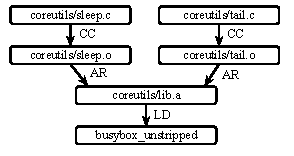
\includegraphics[scale=2.0]{cbg}
\caption{Пример фрагмента команд сборки для апплетов sleep и tail проекта BusyBox.}
\label{figure:cbg}
\end{figure}

% Program fragmentation
Далее выполняется декомпозиция программы при помощи алгоритма конфигурируемой двухэтапной декомпозиции исходного кода программы.

Первым этапом является декомпозиция файлов с исходным кодом на языке Си на модули.
В процессе декомпозиции из всех файлов программы выбираются те, которые требуется верифицировать, и файлы, которые не требуется рассматривать при верификации как, например, тесты и вспомогательные компоненты программы.
На шаге декомпозиции из графа команд сборки $CBG$ выполняется построение двух множеств модулей.
Первое множество модулей $F$ включает все модули программы $F =  \{f_1, ..., f_n\}$, которые могут быть использованы при верификации, но необязательно должны быть верифицированы.
Второе множество модулей $T$ состоит из так называемых целевых модулей $T \subseteq F$, которые требуется верифицировать.
Каждый модуль состоит из файлов с исходным кодом на языке Си, причем каждый файл с исходным кодом программы может быть отнесен только к одному модулю.
%Для каждого модуля выполняется сбор вспомогательной информации: команды и опции компиляции, использованные для компиляции файлов, включенных в модуль, модули, от которых зависит данный, определенные на основе графа команд сборки и опций компиляции, функции, которые экспортируются файлами модуля и используются в других модулях.

Для построения множеств модулей предлагается использовать два типа \textit{стратегий декомпозиции}:
\begin{itemize}
    \item \textit{Специальные стратегии}, которые учитывают устройство $CBG$ определенной программы. 
    Например, специальные стратегии могут служить для извлечения в качестве модулей динамически загружаемых модулей ядра Linux \footnote{The Linux kernel: http://www.kernel.org/} или модулей HTTP сервера Apache\footnote{Apache HTTP server project: http://httpd.apache.org/}.
    \item \textit{Универсальные стратегии}, которые не используют какой-либо информации о программе кроме той, которая может быть извлечена автоматически из графа $CBG$ или предоставлена пользователем в качестве конфигурационных параметров. 
    Примером универсальных стратегий могут быть стратегии, которые каждый файл с исходным кодом программы рассматривают как отдельный модуль или все файлы из одной директории рассматривают как отдельный модуль.
\end{itemize}

Универсальные стратегии полезны для того, чтобы начать первичные эксперименты по верификации какого-либо проекта.
На основе опыта, полученного в ходе таких экспериментов, может понятно как реализовать специальную стратегию декомпозиции или специальная стратегия может вовсе не потребоваться.

На этапе декомпозиции не все файлы с исходным кодом следует отнести к модулям.
Файлы реализаций библиотек, которые содержат неподдерживаемые инструментом верификации конструкции, может потребоваться отфильтровать и заменить моделями окружения.

Следующий этап декомпозиции программы --- аггрегация модулей.
Аггрегация позволяет оптимальным образом подобрать набор модулей, которые требуется включить в качестве зависимостей для верификации каждого целевого модуля.
Как и фрагментацию выполнение аггрегации предлагается осуществлять при помощи \textit{аггрегирующих стратегий}.
В качестве входных данный стратегия получает множества модулей $F$ и $T$, а в качестве результата работы генерируется множество аггрегаций $A$.
Каждая аггрегация $\Delta \in A$ состоит из модулей $\Delta \subseteq F$ где в каждой аггрегации есть хотя бы один целевой модуль $\Delta \cap T \neq \emptyset$.
Подготовка аггрегаций с минимальным числом модулей может привести к росту трудозатрат на моделирование окружения.
В то же время, модули зависят друг от друга и цепочки зависимостей могут быть достаточно длинными, поэтому включение всех модулей из числа зависимостей может отрицательно сказаться на времени работы и возможности верификации исходного кода файлов из модулей аггрегации.

Как и в случае со стратегиями декомпозиции стратегии аггрегации могут быть специальными и универсальными.
В первом случае аггрегации опираются на знание об устройстве верифицируемой программы, заложенное при разработке стратегии.
А универсальные стратегии позволяют выполнять аггрегацию модулей для произвольной программы.
Простейшие универсальные стратегии аггрегации могут выбирать в аггрегацию строго указанные пользователем модули, включать зависимости до выполнения определенного ограничения, например до достижения максимально допустимого размера аггрегации.
Специальные стратегии могут использовать также и дополнительную информацию как, например, информацию о верификационном покрытии модулей для включения в аггрегацию более релевантных модулей.

При реализации стратегий предлагается учитывать различные конфигурационные параметры при генерации аггрегаций, чтобы пользователь мог настроить размер аггрегации или, например, отфильтровать или включать определенные модули.
На практике может потребоваться модифицировать стратегию определенным образом, поэтому реализации стратегий должны быть выполнены таким образом, чтобы модификация и переиспользование имеющихся стратегий было не слишком трудоемким.

В главе, посвященной реализации данного метода, будут рассмотрены примеры стратегий декомпозиции и стратегии аггрегации, реализованные для верификации конкретных программных систем.

\nsubsubsection{Моделирование окружения}
Под моделью окружения далее понимаются фрагменты кода на языке Си, которые будут добавлены в определенную аггрегацию при помощи инструментации исходного кода модулей.
Однако, описывать модель окружения на языке Си не всегда удобно, так как при верификации программы на соответствие разным требованиям и при использовании разных инструментов статической верификации требования к такому коду могут существенно меняться.
Например, при проверке требования, формализованного при помощи задачи достижимости, код модели окружения должен быть последовательным, а при проверке отсутствия состояний гонок модель окружения может быть параллельной.
Ниже модель окружения предлагается описывать в виде системы переходов и на основе данного описания генерировать исходный код модели окружения на языке Си.

Набор препроцессированных файлов с исходным кодом модулей, образующих аггрегацию, обозначим программой $P$.
Для простоты будем рассматривать, что программа содержит некоторый набор глобальных переменных и определений функций $P = < V_p, F_p>$.
Для простоты также не будет рассматриваться вопрос об области видимости переменных и функций.
Обозначим модель окружения программы $P$ как $M$.
\[ M = <F_e, V_e, E > \]
$F_e$ и $V_e$ это вспомогательные определения функций и глобальных переменных, которые являются частью модели окружения, и подготовлены пользователем заранее на языке Си.
Множества функций $F_e$ и $F_p$ могут пересекаться и при генерации верификационной задачи должны будут быть выбраны определения $F_e$, а аналогичные определения $F_p$ должны быть удалены при инструментации исходного кода.
$E$ это описание сценариев, которые может выполнять модель окружения.
$E$ представляет собой параллельную композицию сценариев:
\[ E = \varepsilon_0 \parallel \varepsilon_1 \parallel \varepsilon_2 || \parallel ... \parallel \varepsilon_n \]
Каждый сценарий это система переходов:
\[ \varepsilon_i = <\mathcal{V}_i, \mathcal{A}_i, \alpha^i_0 ,\mathcal{R}_i>\]
Каждая система имеет состояния, которые определяются множеством переменных состояния сценария $\mathcal{V}_i$, которое не пересекается ни с множеством переменных программы, ни с множеством переменных модели окружения, ни с переменными состояния других сценариев:
$\mathcal{V}_i \cap V_p = \emptyset$ и $\forall \varepsilon_i, \varepsilon_j: \mathcal{V}_i \cap \mathcal{V}_j = \emptyset$.
Множество состояний явным образом не описывается, а описываются переходы из состояния в состояние - действия.
$\mathcal{A}_i$ это набор действий, из которых состоит сценарий, а $\mathcal{R}_i:~ \mathcal{A}_i~\times~\mathcal{A}_i$ это отношение переходов, описывающее какие действия могут следовать друг за другом.

Первое действие сценария это $\alpha^i_0$, а последующие определяются отношением переходов $\mathcal{R}_i$. 
Выделяется 3 типа действий: \textit{прием} и \textit{отправка} сигналов и \textit{базовый блок}.
Базовый блок это тройка $\alpha^i_k$:
\[\alpha^i_k = <\varphi^i_k, \beta^i_k, \psi^i_k> \]
Где $\beta^i_k$ содержит базовый блок кода на языке Си, состоящий из инструкций над переменными $\mathcal{V}_i \cup V_p \cup V_e$ с вызовами функций из $F_p$ и $F_e$.
В базовых блоках должен быть корректный код, то есть не должно быть незаконченного кода операторов ветвления и циклов.
Операторы переходы по меткам goto также использовать нельзя.
Логические выражение $\varphi^i_k$ и $\psi^i_k$ над переменными $\mathcal{V}_i \cup V_p \cup V_e$ описывают пред- и постусловия для базового блока.

Прием и отправка сигналов моделируют передачу значений между переменными сценариев.
Рассмотрим сценарий-отправитель $\varepsilon_i$ и сценарий-получатель $\varepsilon_j$ из параллельной композиции $\varepsilon_i \parallel \varepsilon_j$.
Действием отправки сигнала является $\alpha^i_m \in \mathcal{A}_i$, а соответствующим действием приема данного сигнала будет $\alpha^j_n \in \mathcal{A}_j$:
\begin{align*}
&\alpha^i_m = <\varphi^i_m, \varepsilon^i_m, l_m>
&\alpha^j_n = <\varphi^j_n, \pi^j_n, l_n, \psi^i_m>    
\end{align*}
Логические выражения $\varphi^j_n$ и $\psi^j_n$ определены на множестве переменных $\mathcal{V}_j \cup V_p \cup V_e$ и, как и для базового блока, описывают предусловие и постусловие приема сигнала.
Предусловие посылки сигнала является логическим выражением $\varphi^i_m$, определенным на множестве переменных $\mathcal{V}_i \cup V_p \cup V_e$.
Два вектора из переменных $\varepsilon^i_m: {v^i_1, ..., v^i_k}$ где $t = 1..k, v^i_t \in \mathcal{V}_i$ и $\pi^j_n: {v^j_1, ..., v^j_k}$ где $t = 1..k, v^j_t \in \mathcal{V}_j$ определяют присваивание значений переменных сценария отправителя в переменные сценария получателя:
\begin{align*}
&|\pi^j_n| = |\varepsilon^i_m| = k 
&\forall t = 0..k:~v^j_t := v^i_t
\end{align*}
Типы данных переменных должны либо совпадать, либо допускать преобразование друг в друга.
Передача сигналов возможна только тогда, когда действия обозначены метками $l_m = l_n$, которые являются константами и известны заранее.

Семантика выполнения каждого сценария в отдельности достаточно проста.
Сценарий описывает последовательности выполнения кода базовых блоков, гарантируя при этом выполнение соответствующих предусловий и постусловий.
Посылки сигналов на выполнение сценария не влияют, так как, если посылка может произойти, то значения переменных не изменяются, а если не может произойти, то такой сценарий не может выполнить это действие и, если других действий не предусмотрено отношением переходов, то никакие действия далее не будут выполняться сценарием.
Прием сигнала может также вести либо к бесконечному ожиданию, либо получению новых значений переменных состояния.

Для генерации модели окружения из параллельной композиции необходимо определить семантику самой параллельной композиции и передачи сигналов, которые могут происходить в данной параллельной композиции.
Предлагается использовать разные семантики и соответственно разные трансляторы модели окружения на язык Си.
Так, например, для генерации последовательного кода семантика будет одной, а при использовании потоков POSIX можно сгенерировать модель окружения с другой семантикой.

В тоже время в любой семантике в параллельной композиции должны быть выполнены следующие требования:
\begin{itemize}
    \item Все сценарии и метки сигналов определены заранее. Сценарии не порождаются и не могут быть удалены. Заранее указанные метки позволяют также перед генерацией кода определить всех возможных получателей и отправителей сигналов в модели окружения.
    \item Только один сценарий в композиции может иметь в качестве первого действия $\alpha^i_0$ действие с типом базового блока. 
    Это требование упрощает генерацию функции точки входа, с которой инструмент верификации начнет анализ модели окружения.
    Остальные сценарии должны иметь в качестве первого действия прием сигнала, то есть ожидать приема сигнала перед выполнением каких-либо действий.
    \item Вызов функций из $P$ должен рассматриваться как возможная посылка сигнала определенному сценарию. 
    Для этого можно ввести новый тип действия, но этот случай не рассмотрен для краткости.
    Семантика такого сигнала заключается в том, что программа после вызова функции из окружения может инициализировать выполнение окружением определенных действий, которые сценарий, получающий сигнал, моделирует.
\end{itemize}

Ниже мы рассмотрим метод генерации модели окружения ее трансляцию на язык Си. 
Схема генерации модели окружения представлена на рисунке \ref{figure:em}.
Для генерации модели используются один или несколько генераторов сценариев модели окружения.
Сгенерированные сценарии образуют промежуточную модель окружения, которая и является параллельной композицией.
Затем транслятор в соответствии с заданной пользователем конфигурацией генерирует код модели окружения на языке Си.

\begin{figure}
\centering
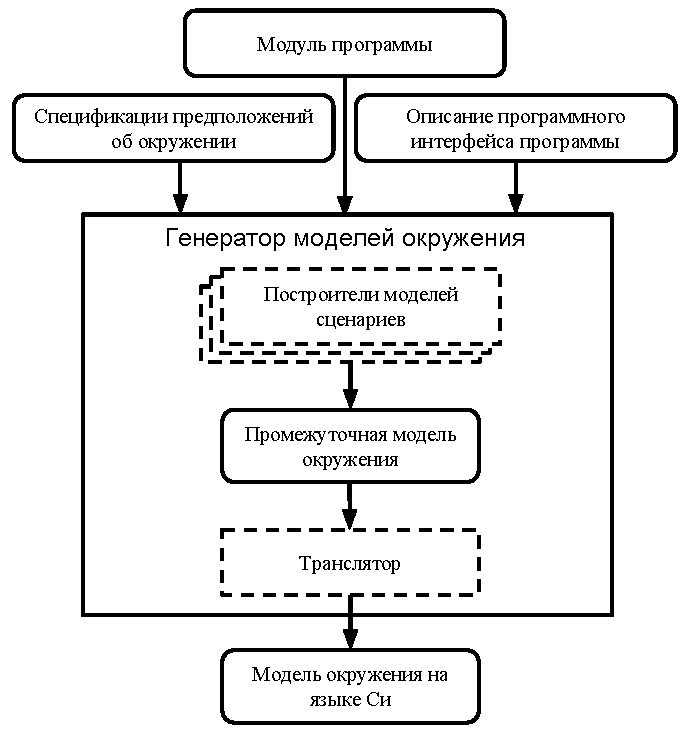
\includegraphics[scale=1.2]{generators}
\caption{Генерация модели окружения.}
\label{figure:em}
\end{figure}

В качестве входных данный каждый генератор получает аггрегацию и спецификации, подготовленные вручную пользователем при необходимости.
Данные спецификации могут представлять собой набор конфигурационных параметров для генератора или полноценное описание модели окружения на языке предметной области.
Генераторы подготавливают сценарии для параллельной композиции независимо друг от друга или образуя цепочки.

Программа использует разные интерфейсы и частично может их реализовывать.
Предлагается генерировать сценарии в зависимости от интерфейсов, которые требуется моделировать.
Генератор может анализировать исходный код аггрегации для выявления используемых интерфейсов, чтобы определить когда и какие сценарии требуется генерировать.
Например, функция main тоже является интерфейсом.
Простейший генератор может определить, что аггрегация содержит данную функцию и сгенерировать сценарий, который может вызывать данную функцию с различными параметрами.

Транслятор генерирует код на основе промежуточной модели окружения, исходного кода аггрегации и конфигурационных параметров, заданных пользователем.
Генерация производится в соответствии с определенной реализованной семантикой операции параллельной композиции и пересылки сигналов.

В некоторых случаях генератор может накладывать дополнительные ограничения на то, какие сценарии может содержать промежуточная модель окружения.
На практике инструменты статической верификации не позволяют использовать произвольный код на языке Си, так как слишком сложная модель окружения будет лишь затруднять верификацию программы.
При реализации транслятора используется такая семантика, чтобы трассово-эквивалентный параллельной композиции сгенерированный код мог быть верифицирован.
Например, требовать, чтобы прием сигнала мог происходить только в первом и любом последнем действиях сценария.

Отметим, что для контроля за пред- и постусловиями удобно использовать механизм, поддерживаемый инструментами статической верификации для моделирования окружения, который позволяет не рассматривать пути при верификации, на которых не выполняется или наоборот --- выполняется та или иная формула, заданная в виде аргумента специальной модельной функции.
Данный механизм был рассмотрен в первой главе ранее.
Без использования данного механизма задача трансляции сценариев представляется гораздо более сложной задачей.

При генерации модели окружения транслятор может использовать определенные наборы функций и переменных, реализованных пользователем.
Ранее они обозначались как $F_e$ и $V_e$.
На практике такие модели служат для выполнения определенных операций в зависимости от программы.
Например, для выделения памяти в модели окружения удобно иметь разные наборы моделей, так как инструменты верификации могут иметь разные наборы функций, которые инструмент моделирует самостоятельно.
Также при верификации операционных систем и пользовательских программ наборы таких функций могут быть разными.

\nsubsubsection{Генерация верификационных задач}
После того, как для каждой аггрегации была сгенерирована модель окружения, начинается процесс генерации верификационных задач для каждой аггрегации.
Для каждой тройки аггрегации, модели окружения и правила корректности генерируется отдельная верификационная задача.
Верификационные задачи предлагается готовить согласно формату соревнований SV-COMP.

Для формализации правил предлагается использовать тот же подход, который изложен в диссертации~\cite{NovikovDisser} и опробирован в системе статической верификации LDV Tools.
Данный подход сформулирован для интерфейса драйверов, но без изменения может быть применен для формализации специальных правил корректности в виде контрактных спецификаций.
Пользователь может разработать контрактные спецификации для проверки требуемого специального правила корректности, затем для заданной аггрегации будет сгенерирован код формализованного правила на языке Си и спецификация свойства корректности.

Код модели окружения и код формализованного правила на языке Си при помощи инструментируются в препроцессированные файлы с исходным кодом аггрегации.
Подготовленный препроцессированный инструментированный код и спецификация свойства корректности становятся основой верификационной задачи.
Дополнительные сведения для верификационных задач, как, например, параметры для запуска инструмента статической верификации и максимальные ограничения на доступные вычислительные ресурсы задаются пользователем для всех верификационных задач единообразно.  

\nsubsubsection{Масштабируемое решение верификационных задач}
Ниже предлагается метод модульной масштабируемой статической верификации для эффективного использования вычислительных ресурсов при верификации.

И генерация верификационных задач, и их решение при помощи инструментов статической верификации требует большого объема процессорного времени, оперативной и дисковой памяти.
Для получения воспроизводимых и корректных результатов требуется гарантировать, что генерация и решение верификационных задач выполняются изолированно друг от друга и для их решения доступен достаточный объем вычислительных ресурсов.
В то же время генерация и решение верификационных задач должны выполняться параллельно с возможностью эффективно использовать возможности вычислительной системы и экономить ее вычислительные ресурсы в условиях, когда объем реально необходимых вычислительных ресурсов неизвестен.

Назовем совокупность данных для запуска компонентов верификационной системы для генерации верификационных задач в рамках верификации определенной программы  \textit{верификационным заданием}, а процесс генерации верификационных задач --- \textit{решением верификационного задания}.
Компонент \textit{планировщик} выполняет как решение верификационных заданий, так и решение верификационных задач.
Генерация верификационных задач может требовать значительного количества времени.
По этой причине предлагается начинать решать верификационные задачи по мере их поступления, если имеются свободные вычислительные ресурсы.
Для решения нескольких задач предлагается использовать одну рабочую станцию, удовлетворяющую необходимым минимальным системным требованиям для выполнения статической верификации.
Для решения больших наборов задач и сокращения времени на верификацию предлагается использовать IaaS облачную платформу или кластер.

Планировщик в таком случае выполняет мониторинг доступных вычислительных ресурсов, распределяет верификационные задачи и задания между вычислительными узлами и контролирует их выполнение.
Требуемые максимальные ограничения на вычислительные ресурсы, которые требуется резервировать для решения верификационной задачи, определяются пользователем.
Планировщик должен резервировать требуемый объем ресурсов при решении соответствующей верификационной задачи или задания.
Также планировщик должен поддерживать отмену верификационных задач и заданий по требованию пользователя.

Некоторые верификационные задачи могут требовать гораздо меньше вычислительных ресурсов, чем пользователь указывает в качестве максимального ограничения при запуске верификационного задания.
Чтобы избежать резервирования слишком большого объема вычислительных ресурсов при решении верификационных задач планировщик может реализовывать алгоритмы для экономии вычислительных ресурсов и запуска задач с меньшими ограничениями на вычислительные ресурсы.
Данные ограничения можно рассчитывать на основе статистики решения других верификационных задач, которые используют тот же инструмент верификации и проверяют те же правила корректности.
Те задачи, которые имели уменьшенные ограничения на вычислительные ресурсы, но которые все же превысили данные ограничения, требуется решить заново для получения воспроизводимых и корректных результатов верификации.

В случае использования облачного сервиса или вычислительного кластера планировщик должен поддерживать подключение и отключение вычислительных узлов динамически.
Если вычислительный узел неожиданно перестает быть частью вычислительного кластера, то верификационные задачи и задания, решаемые на данном узле, должны быть решены заново на других доступных узлах.
Если же узлов с подходящими характеристиками нет, то верификационное задание должно быть отменено с указанием советующего сообщения об ошибке.

\nsubsubsection{Анализ результатов верификации}
После генерации верификационных задач и их решения требуется выполнить валидацию результатов и анализ срабатываний на предмет их ложности.
Для этого для каждой верификационной задачи извлекается необходимая информация, которая затем должна быть предоставлена пользователю.
Пользователь анализирует результаты при помощи пользовательского интерфейса.

Для каждой верификационной задачи предлагается извлекать вердикт, отчет о затраченных вычислительных ресурсах, свидетельство корректности или нарушения, журнал выполнения инструмента статической верификации и вспомогательную информацию такую, как, например, верификационное покрытие или статистику для внутреннего представления модели программы.
Так как свидетельства нарушения, которые генерируют инструменты статической верификации могут не содержать некоторых важных с точки зрения экспертизы пользователя деталей, то перед визуализацией свидетельств корректности предлагается добавлять некоторую дополнительную информацию.

Кроме информации об исходном коде программы при визуализации свидетельств нарушения предлагается добавлять сведения о сгенерированной модели окружения.
Например, снабжать вызовы функций из модели окружения вспомогательными комментариями с пояснениями что именно моделирует модель.

После решения верификационного задания отчеты о верификационном покрытии при верификации программы могут быть сведены воедино для визуализации итогового отчета о верификационном покрытии для всей программы.
При верификации программы на соответствие нескольким правилам корректности предлагается подготавливать независимые отдельные отчеты об итоговом верификационном покрытии, так как при проверке разных правил могут использоваться разные модели окружения и различные инструменты статической верификации или их конфигурации.


Для автоматизации анализа результатов пользовательский интерфейс должен предоставлять следующие возможности:
\begin{itemize}
\item Показывать информацию о всех запущенных и решенных верификационных заданиях.
Для каждого задания должны быть доступны параметры, с которыми выполнялся запуск соответствующих верификационных заданий, включая спецификации для генерации моделей окружения и спецификации для формализации правил корректности.
Для решенных верификационных заданий пользователь должен видеть прогресс решения --- число верификационных задач, которые требуется подготовить и решить, и число задач, которые уже решены и результат решения которых может быть проанализирован.
\item Визуализировать данные о решении верификационных задач, которые трудно анализировать пользователю в <<сыром>> виде.
К таким данным относятся свидетельства корректности и нарушения, отчеты о верификационном покрытии.
\item Предоставлять статистику о решении верификационного задания и о результате экспертизы результатов.
Для каждого решенного верификационного задания предлагается указать число срабатываний, число верификационных задач, которые считаются корректными, общее число верификационных задач, число аггрегаций, для которых не удалось сгенерировать верификационную задачу и классификацию соответствующих проблем.
\item Для каждого срабатывания или доказательства корректности пользователь должен иметь возможность указать экспертную оценку и атрибуты, при которых данная экспертная оценка может быть перенесена автоматически для других верификационных заданий.
Например, если разные задания содержат одну и ту же ошибку, найденную инструментами статической верификации, то экспертная оценка может быть автоматически применена к обоим заданиям, если ошибочный путь, правило корректности и другие атрибуты совпадают.
В то же время пользователь должен иметь возможность подтверждать или отменять автоматическое применение экспертных оценок.
\item Для каждого задания предлагается хранить историю изменений параметров задания, а для каждой экспертной оценки историю изменения оценки пользователями.
\item Предлагается визуализировать данные в зависимости от ролей каждого пользователя, работающего с системой статической верификации.
Так, например, инженер, настраивающий и запускающий процесс верификации может быть более заинтересован в проблемах генерации задач и случаях, когда вердикт не может быть получен, а эксперты, выполняющие экспертизу, заинтересованы прежде всего в создании экспертных оценок и просмотре статистики.
\item Представлять результаты верификации по мере их появления. 
Процесс конфигурирования системы статической верификации может быть достаточно сложным, поэтому важно на раннем этапе обнаружить наличие каких-либо проблем и отменить некорректно настроенное решение верификационного задания, не дожидаясь его завершения.
\end{itemize}

Для выполнения экспертизы ошибочных путей, являющихся частью сертификатов нарушения свойств корректности, предлагается предварительно выполнить некоторые преобразования.
Так как согласно формату SV-COMP формат свидетельств является только машиночитаемым.

Для этого был разработан формат для свидетельств нарушения свойств корректности, который не меняя формат по содержанию требует сохранять в сертификате свидетельства больше информации, которая необходима для экспертизы.
Данный формат может быть реализован в одном инструменте статической верификации, который может использоваться и как валидатор сертификатов.
Сертификаты других инструментов статической верификации могут быть поданы на вход данному инструменту для валидации и переведены в требуемый формат.
В таком случае остается возможность использовать один инструмент статической верификации для вывода сертификатов в нужном формате, а другие для выполнения непосредственно верификации.

При визуализации свидетельств корректности в предложенном формате предлагается также сопровождать ошибочные пути оригинальным исходным кодом программы, моделей окружения и кодом для формализации правила корректности.
Так как верификационная задача содержит препроцессированный и инструментированный код программы, который может быть сложен для анализа пользователем.
Также предлагается сопровождать ошибочные пути вспомогательной информацией о модели окружения и правиле корректности, которая может быть получена из соответствующих спецификаций, разработанных пользователем.

\nsubsection{Глава 3}
% Ожидается в сумме 10 страниц
% Глава 3 Реализация метода статической верификации программ на языке Си 
Ниже описана архитектура системы статической верификации Klever, в рамках которой был реализован предложенный метод масштабируемой модульной статической верификации программ на языке Си.

Предложенный метод реализован в системе статической верификации Klever предназначенной для статической верификации программ на языке Си с расширениями GNU\footnote{https://forge.ispras.ru/projects/klever}.
Klever является проектом с открытым исходным кодом.
Основной язык разработки системы Python 3.4.
Система Klever может быть установлена и использована на различных дистрибутивах операционной системы Linux.
Система может быть автоматически развернута и использована в облачной IaaS платформе OpenStack.

Система состоит из 3 основных взаимодействующих компонентов: пользовательского интерфейса Bridge, генератора верификационных задач Core и решателя Scheduler. 

\nsubsubsection{Генерация верификационных задач}
Core позволяет генерировать верификационные задачи параллельно для ускорения всего процесса верификации.
Для выполнения контролируемой сборки и перехвата команд компиляции используется проект Clade\footnote{https://github.com/17451k/clade}.
Для выполнения запросов к исходному коду и инструментации исходного кода используется CIF~\cite{Novikov2013}.
CIF это инструмент для инструментации, основанный на GCC, поэтому он в достаточной степени поддерживает инструментацию программ на языке Си с расширениями GNU.
CIF позволяет выполнять различные запросы к исходному коду программ для получения информации о макросах, функциях и глобальных переменных.
При инструментации инструмент позволяет добавлять код в начало или в конец файлов на языке Си, а также заменять вызовы функций и макроподстановки.

При верификации поддерживается проверка либо специальных правил корректности, либо правил безопасного программирования, включая корректную работу с памятью и отсутствие состояний гонок.
Система позволяет расширять набор правил либо за счет формализации правил в качестве задачи достижимости, либо за счет встроенной поддержки нового правила инструментом статической верификации.

Core выполняет декомпозицию исходного кода, генерацию моделей окружения и  формирование верификационных задач в соответствии с форматом SV-COMP, поддерживаемом инструментами статической верификации.
Сгенерированные задачи загружаются в компонент Bridge и передаются на решение компоненту Scheduler.

Core реализует методы декомпозиции программы, генерации моделей окружения и инструментации кода модуля верифицируемой программы для получения верификационных задач.
Архитектура данного компонента поддерживает параллельную работу на каждом этапе для ускорения работы с большим числом модулей, которые нужно проверить на соответствие нескольким требованиям.
В архитектуре данного компонента возможно использование расширений для добавления к уже имеющимся компонентам их модификаций для адаптации процесса генерации верификационных задач к работе над с определенной программной системой.
Например, система статической верификации позволяет добавлять стратегии декомпозиции кода, генераторы и трансляторы модели окружения на язык Си, а также встраивать дополнительные компоненты для выполнения новых действий в процесс генерации верификационных задач, чтобы облегчить статическую верификацию разных программных систем на соответствие разным наборам требований с использованием разных инструментов статической верификации.

Так для верификации модулей ядра Linux была реализована одна стратегия декомпозиции исходного кода.
Данная стратегия формирует каждый фрагмент из файлов с исходным кодом одного динамически загружаемого модуля ядра Linux.
Для аггрегации были реализованы три стратегии:
\begin{itemize}
    \item Стратегия, которая включает в каждую аггрегацию только один фрагмент.
    Данная стратегия использовалась в подавляющем числе экспериментов.
    \item Стратегия, которая рекурсивно добавляет в аггрегацию модули на основе требований по загрузке модулей в память.
    Данная стратегия не подтвердила своей эффективности из-за высокой сложности аггрегаций для инструментов статической верификации.
    \item Стратегия, формирующая аггрегации на основе описания, подготовленного пользователем вручную.
    Данная стратегия применялась для более точной верификации отдельных модулей.
\end{itemize}

Для генерации моделей окружения для модулей ядра Linux использовался схожий подход, с реализованным ранее в системе статической верификации LDV Tools, но с существенными отличиями в реализации~\cite{ZakharovEnv2015}.
Для генерации моделей окружения были реализованы два генератора сценариев для промежуточной модели окружения.
Один из генераторов на основе данных, полученных при анализе исходного кода модулей и вручную подготовленных спецификаций на языке предметной области, генерирует модели окружения, отвечающие за вызов обработчиков драйверов, регистрируемых в подсистемах ядра.
Другой генератор выполняет вызов функций инициализации и выхода модулей, включенных в аггрегацию, согласно возможному их порядку загрузки в память.
Данный порядок определяется за счет решения задачи топологической сортировки графа зависимостей модулей.

Для трансляции промежуточной модели окружения на язык Си был реализован соответствующий транслятор согласно предложенному методу.
Транслятор генерирует код в нотации аспектно-ориентированного расширения языка Си для последующей инструментации модели окружения в исходный код модулей при помощи CIF.
Транслятор модели окружения позволяет генерировать либо последовательный код, либо параллельный код с использованием интерфейса POSIX для работы с потоками.
Подобной модели окружения достаточно для поиска гонок по данным в параллельном коде ядра операционной системы, где процессы выполняются в общем адресном пространстве.
Для моделирования некоторых общих интерфейсов ядра, широко используемых модулями, были также подготовлены модели непосредственно на языке Си.

Для верификации подсистем ядра Linux была реализована дополнительная стратегия для объединения файлов подсистемы ядра в один модуль, а загружаемых модулей ядра Linux в другие фрагменты.
Данная стратегия позволяет верифицировать как подсистему отдельно от модулей, которые используют интерфейсы подсистемы, так и вместе с ними.
Для реализации этого режима была также реализована соответствующая стратегия для аггрегации модулей.

Еще одна стратегия аггрегации, реализованная для статической верификации подсистем ядра Linux, автоматизирует выбор модулей для верификации подсистемы на основе верификационного покрытия, полученного при верификации динамически загружаемых модулей отдельно.
Такая стратегия существенно облегчает поиск таких модулей для верификации интерфейсов подсистемы ядра, для которых генерируемая модель окружения позволяет достигнуть требуемого верификационного покрытия.

Еще одна стратегия для аггрегации, используемая для верификации подсистем на основе вручную заданного списка файлов подсистемы и загружаемых модулей, использовалась и при верификации модулей отдельно.

Для корректного моделирования окружения подсистем ядра использовался генератор для генерации вызова обработчиков, так как подсистемы реализуют обработчики аналогично модулям ядра, а также генератор для инициализации подсистем.
Последний упомянутый генератор генерирует вызовы функций инициализации подсистемы согласно уровню иерархии подсистем в ядре Linux, который пользователь предоставляет в виде конфигурации для генератора.
Сами функции инициализации определялись автоматически на основе результата анализа исходного кода.

Для трансляции промежуточной модели окружения на язык Си использовался уже тот же  транслятор, что и применялся для верификации загружаемых модулей ядра Linux.
При верификации использовался расширенный набор моделей интерфейсов ядра Linux, подготовленный вручную на языке Си, для корректного моделирования механизма kernel panic и отсутствия запланированного завершения работы подсистемы, так как подсистемы работают вплоть до завершения работы операционной системы, поэтому никогда не освобождают некоторые ресурсы и память явным образом.

Для поддержки верификации пользовательских программ были реализованы несколько универсальных стратегий декомпозиции и аггрегации.
Для верификации апплетов Busybox для декомпозиции апплетов на модули использовалась простейшая стратегия, ставящая в соответствие одному модулю один файл.
Для генерации аггрегаций использовалась специальная стратегия для работы с Busybox:
\begin{itemize}
    \item Стратегия добавляет в аггрегацию строго один модуль с функцией main апплета.
    \item Согласно конфигурации, стратегия добавляет в аггрегацию остальные модули, реализующие функциональность апплета.
    \item Также в зависимости от конфигурации стратегия добавляет вспомогательные файлы, используемые файлами апплета из библиотеки libbb.
    \item Конфигурация позволяет указывать конкретные файлы, модули с которыми никогда не добавляются в аггрегации или наоборот --- добавляются в каждую аггрегацию.
\end{itemize}

Для генерации модели окружения использовался генератор для вызова экспортируемых функций из аггрегации.
В данном случае генератор вызывал лишь функцию main из апплета с неопределенными параметрами для моделирования вызова апплета с разными параметрами командной строки.

Для верификации пользовательских программ были подготовлены модели некоторых функций стандартной библиотеки языка Си из заголовочных файлов "string.h" и "stdio.h".
Для верификации BusyBox были также разработаны модели некоторых функций библиотеки libbb, которые вызывали затруднения при анализе инструментом статической верификации.

\nsubsubsection{Решение верификационных задач и заданий}

Компонент Scheduler предназначен для запуска экземпляров компонента Core, генерирующих верификационные задачи, и инструментов статической верификации, выполняющих решение сгенерированных верификационных задач.
Данный компонент осуществляет контроль за доступностью и потреблением вычислительных ресурсов и гарантирует изолированную работу данных компонентов.
Scheduler осуществляет планирование и распределение ресурсов, чтобы избежать нехватки вычислительных ресурсов или неэффективного использования аппаратуры.

Для выполнения верификации пользователи должны указать для каждого доступного вычислительного узла системы доступные для выполнения верификации вычислительные ресурсы такие, как число ядер CPU, объем оперативной памяти и дискового пространства.
При этом на вычислительных узлах должно быть достаточно вычислительных ресурсов для функционирования операционной системы и других запущенных сервисов.

Для изолированного выполнения инструментов статической верификации при решении верификационных задач и для измерения затраченных вычислительных ресурсов, а также для остановки решения при превышении заданных ограничений, предлагается использовать упомянутый ранее инструмент BenchExec~\cite{Beyer2015}.
Кроме возможностей по контролю и измерению вычислительных ресурсов важным достоинством данного инструмента является наличие адаптеров для инструментов статической верификации.
Как было сказано ранее, данные адаптеры упрощают запуск и первичный анализ результатов верификации.

Для планирования распределения вычислительных ресурсов в процессе статической верификации реализован жадный алгоритм.
Для запуска экземпляров компонента Core и инструментов статической верификации используются отдельные модули, реализующие определенный интерфейс для запуска генераторов верификационных задач и инструментов статической верификации.
Данные модули позволяют использовать для статической верификации один вычислительный узел, распределенную вычислительную систему, а также облачные сервисы, как, например, \mbox{VerifierCloud}.

Для контроля за вычислительными узлами было реализовано три модуля планировщика \mbox{Scheduler}:
\begin{enumerate}
\item \textit{Klever Native Scheduler} для запуска верификации на одном вычислительном узле.
\item \textit{Klever Docker Scheduler} для решения верификационных задач и заданий при помощи распределенной вычислительной системы, управляемой Kubernetes.
\item \textit{Klever VerifierCloud Scheduler} для работы с облачным сервисом VerifierCloud\footnote{https://vcloud.sosy-lab.org/cpachecker/webclient/help/}, позволяющем решать верификационные задачи с использованием кластера.
\end{enumerate}
Для управления доступными вычислительными узлами используется Consul.

Для решения верификационных задач можно использовать инструменты статической верификации CPAchecker или Ultimate Automizer~\cite{Heizmann2015}.
Для интеграции других инструментов статической верификации требуется:
\begin{enumerate}
\item Для каждого правила корректности, которое требуется проверять при помощи нового инструмента, указать конфигурационные параметры для запуска.
\item Установить данный инструмент на вычислительных узлах таким образом, чтобы \textit{Klever Native Scheduler} мог выполнить запуск инструмента, имея в распоряжении только путь до исполняемого файла в системе.
\item Для \textit{Klever Container Scheduler} подготовить соответствующие Docker образы c установленным инструментом.
\end{enumerate}

\nsubsubsection{Пользовательский интерфейс}

Компонент Bridge решает три ключевые задачи в рамках системы статической верификации Klever:
\begin{itemize}
\item \textit{Взаимодействие с пользователем.}
Пользовательский интерфейс системы статической верификации важен с точки зрения удобства использования системы, так как организация процесса запуска статической верификации и выполнения экспертизы результатов статической верификации, сравнения результатов и организации совместной работы нескольких пользователей с полученными результатами достаточно важна.  
\item \textit{Хранение результатов верификации.} 
В процессе статической верификации накапливаются данные, включая как сгенерированные системой статической верификации, так и подготовленные пользователями. 
К первой категории относятся предупреждения об ошибках, доказательства корректности, информация, полученная в ходе контролируемой сборки программы и т.д.
Результаты требуется хранить достаточно долгое время, так как статическая верификация может требовать много времени и вычислительных ресурсов для воспроизведения результатов. 
Спецификации для моделирования окружения и формализации требований, а также экспертные оценки составляют данные, которые система статической верификации хранит по результатам работы пользователя.
Данная информация может переиспользоваться при верификации разных модулей и версий программы, а также при изменении конфигурации системы и выборе новых инструментов статической верификации. 
\item \textit{Организация взаимодействия между другими компонентами системы}.
В ходе работы между компонентами системы осуществляется достаточно активный обмен данными.
Данный компонент выполняет роль посредника между компонентами и надежного хранилища данных, сгенерированных в ходе работы системы статической верификации.
\end{itemize}

Пользовательский интерфейс \textit{Klever Bridge} разработан на основе фреймворка Django и предоставляет все требуемые методом возможности.
Для хранения данный компонент использует базу данных под управлением PostgreSQL или MariaDB.
В для установки пользователи могут использовать веб серверы Apache2 с mod\_wsgi или NGINX с Gunicorn.

Компонент \textit{Klever Bridge} позволяет использовать систему статической верификации нескольким пользователям с различными ролями, адаптируя представление согласно конфигурационным параметрам и роли каждого пользователя.
Компонент также автоматизирует перенос экспертных оценок между результатами решения схожих верификационных заданий.
Для этого реализовано несколько алгоритмов сравнения свидетельств корректности и автоматизированной разметки сообщений об ошибках на основе регулярных выражений.
Но на данный момент компонент не поддерживает визуализацию свидетельств корректности. 

\nsubsection{Глава 4} 

В данной главе описаны результаты практической апробации системы статической верификации Klever для верификации различного системного программного обеспечения.

При помощи Klever были выполнены эксперименты по верификации нескольких операционных систем и проекта Busybox для подтверждения возможности верификации пользовательских программ.
Ниже представлены некоторые результаты верификации модулей ядра и подсистем ядра Linux и апплетов Busybox.
Результаты верификации других операционных систем не могут быть опубликованы в данной работе из-за запрета о разглашении результатов.

Для декомпозиции исходного кода ядра операционной системы Linux на модули используются специализированные стратегии, позволяющие проверять как загружаемые модули ядра, так и подсистемы ядра.
Для генерации моделей окружения были реализованы два генератора моделей окружения, которые позволяют генерировать модели окружения с вызовом обработчиков и функций инициализации подсистем ядра и динамически загружаемых модулей ядра Linux.
При верификации были переиспользованы контрактные спецификации, разработанные в рамках системы статической верификации LDV Tools, позволяющие проверить корректность использования интерфейсов ядра в модулях ядра Linux.
При верификации использовались инструменты статической верификации CPAchecker и Ultimate Automizer.

Ниже представлены некоторые результаты, полученные при верификации модулей ядра Linux версии 3.14.
Klever генерирует аггрегации для 3821 загружаемых модулей ядра, но для 429 модулей модель окружения не может быть сгенерирована из-за отсутствия функции инициализации.
Верификационное покрытие по строкам исходного кода модулей составляет 48\%, а по функциями 36\%.
Покрытие зависит от полноты и корректности спецификаций для генерации моделей окружения, а также из-за отсутствия генератора для моделирования вызова экспортируемых функций из модулей.

Для генерации моделей окружения были подготовлены спецификации для поддержки драйверов block, class, pci, hid, platform, serial, usb, а также для вызова обработчиков ethernet, file, ieee80211, net device, proto, real time clocks, scsi, sequential, block, tty, urb и моделирования механизмов отложенного выполнения таких, как таймеры, очереди, тасклеты, потоки ядра kthreads, а также для моделирования прерываний.
Прежде всего целью было верифицировать драйверы устройств.
Покрытие для драйверов в среднем соствило в общей совокупности 50\%.

При верификации модули проверялись на соответвие 30 правилам корректности из которых 28 было специальных и правило корректной работы с памятью и отстутвия состояний гонок по данным.

При верификации возникла 301 уникальная проблема из которых 97 связано с отвтутвием моделей некоторых функций ядра а 41 проблема вызвана некорректно сгенерированной моделью окружения.
При верификации система статической верификации Klever позволила обнаружить 150 проблем в модулях ядра Linux версии 3.14.
Полный список найденных проблем, подтвержденных разработчиками пополняется на сайте проекта LDV\footnote{http://linuxtesting.org/results/ldv}.

Детальные результаты верификации подсистем ядра Linux представлены в работе~\cite{Novikov:2018:ISOLA}.
В рамках данной работы выполнялась верификация подсистем CHAR, TTY и GPIO ядер версий начиная с 3.14 по 3.19 как вместе так и без динамически загружаемых модулей.
При верификации проверялись 11 специальных правил корректности и корректная работа с памятью.
В среднем верификационное покрытие по функциям в подсистемах TTY и CHAR составило 80\% и в подсистеме GPIO iсоставило 60\%. 
При верификации новые ошибки обнаружить не удалось.
Из срабатываний снитрумента статической верификации 62\% являлись ложными срабатываниями из-за неточной модели окружения и 38\% были проблемами в модулях, с которыми верифицировались данные подсистемы.
Для подтверждения возможности обнаружения ошибок в подсистемах ядра было выбрано 8 ошибок, исправленных в указанных подсистемах. 
Из них удалось обнаружить 4: b5325a02aa84, e9595f84a627, 00acc3dc2480 и
07584d4a356e из репозитория linux-stable\footnote{http://git.kernel.org/pub/scm/linux/kernel/git/stable/linux.git}.

При верификации проекта BusyBox версии 1.28.3 собранном в конфигурации defconfig было верифицировано 185 апплетов.
Аггрегации были сгенерированы полностью автоматически со всеми зависимостями из библиотеки libbb кроме 4 файлов, исключенных из-за высокой сложности для инструмента статической верификации.
Покрытие по строкам в верифицированных файлах составило  93\% и по функциям 86\%.
При верификации было найдено 2 утечки памяти, которые намеренно были допущены разработчиками.
Еще было выдано 27 ложных срабатываний из которых 14 вызваны недостаточно точными моделями функций стандартной библиотеки языка Си и 11 неточным анализом инструмента статической верификации.

\nsubsection{Заключение}
Основные научные результаты, полученные в данной работе, состоят в следующем:
\begin{itemize}
    \item Был разработан метод модульной масштабируемой статической верификации программ на языке Си с расширениями GNU.
    Метод позволяет автоматизировать весь процесс верификации программы, включая подготовку исходного кода, декомпозицию программы, моделирование окружения, запуск инструментов статической верификации и анализ результатов.
    \item Был разработан алгоритм конфигурируемой двухэтапной декомпозиции исходного кода программ на языке Си. 
    \item Был предложен способ описания моделей окружения программ на языке Си при помощи параллельной композиции систем переходов и основанный на данной модели алгоритм генерации моделей окружения модулей программ на языке Си.
    \item Был разработан метод масштабируемой модульной статической верификации программ при помощи распределенных вычислительных систем и облачных сервисов.
    \item Была предложена архитектура системы статической верификации для реализации предложенного метода, которая была реализована в системе статической верификации программ на языке Си Klever.
    \item Были проведены эксперименты для оценки применимости метода для верификации программ на языке Си. Результаты экспериментов подтвердили возможность проведения масштабируемой модульной статической верификации различных программных систем, включая пользовательские программы и операционные системы, в рамках предложенного метода.
    
\end{itemize}

% ----------------------------------------------------------------
\printbibliography[heading=authorcited,keyword={mypaper}, resetnumbers=true]
\printbibliography[heading=cited, notkeyword={mypaper}]

% ----------------------------------------------------------------
% Пример выходных данных
%\clearpage
%\thispagestyle{empty}
%\normalfont\selectfont
%\vspace*{2cm}
%\begin{center}
%\textit{Научное издание}\\
%\vskip 2cm
%\makeatletter
%\@author
%\vskip 1.5cm
%\@title{} на тему:\\
%\@topic\\
%\makeatother
%\end{center}
%\vfill
%Подписано в печать~25.01.2011.
%Формат~$60 \times 90$~1/16.
%Тираж~100~экз.
%Заказ~256.\\[2ex]
%\noindent
%Санкт-Петербургская издательская фирма <<Наука>> РАН.
%199034, Санкт-Петербург, Менделеевская линия, 1,
%\href{http://www.naukaspb.spb.ru}{http://www.naukaspb.spb.ru}
\end{document}
